\documentclass[sigplan,11pt,nonacm]{acmart}
\settopmatter{printfolios}

\usepackage{booktabs} % For formal tables
\usepackage{subcaption}
\usepackage{tikz}
\usetikzlibrary{fit}
\usepackage{pgfplots}
\usepackage{pgfplotstable}
\usepackage{hyphenat}
\usepackage{todonotes}
\usepackage[babel]{csquotes}
\usepackage{listings}
\lstset{frame=tb,
  % language=Rust,
  aboveskip=3mm,
  belowskip=3mm,
  showstringspaces=false,
  columns=flexible,
  basicstyle={\small\ttfamily},
  numbers=left,
  numbersep=5pt,
  xleftmargin=\parindent,
  numberstyle=\color{gray},
  % keywordstyle=\color{blue},
  % commentstyle=\color{dkgreen},
  % stringstyle=\color{mauve},
  breaklines=true,
  breakatwhitespace=true,
  tabsize=2
}
\pagenumbering{gobble}
\definecolor{cgreen}{RGB}{60,201,65}



\begin{document}
\title{Ownership types in theory and practice (in Rust)}
\author{Fritz Rehde}
\affiliation{%
  \institution{Technical University of Munich}
  \country{Germany}
}
\email{fritz.rehde@tum.de}

\begin{abstract}
% Abstract: Brief summary of area, problem, approach, key result

Object aliasing is the concept of accessing the same memory through different symbolic names in object-oriented programming languages.
Many programming bugs are created through unintentional aliases, which are hard to detect and can lead to unexpected side effects.
Ownership types are one solution that attempts to prevent many alias-related bugs.
The premise of ownership types is that not only the fields of an object are protected from external access, but also all objects stored in those fields.
This is done by allowing objects to take ownership of other objects.

This paper depicts the different kinds of ownership types and explains how the modern programming language Rust uses ownership types.

\end{abstract}

\keywords{Ownership, Type, Safety, Rust}

\maketitle

\section{Introduction}
\label{sec:introduction}
% Introduction: introduce area, problem, approach, key results, contributions, outline

One of the main goals of ownership types is to improve memory safety.
Understanding memory-related bugs will, therefore, help in understanding why ownership types are useful.


\subsection{Memory Safety}
\label{sec:memory-safety}

% TODO: define memory safety
% Memory safety refers to the state of a program where memory pointers or references always refer to valid memory.

The tech giants Google \cite{google-memory-safety} and Microsoft \cite{microsoft-memory-safety} have both revealed that around 70 percent of their vulnerabilities were the result of memory safety issues.
The importance of memory safety is further underlined by the fact that the National Security Agency of the United States of America has published a Cybersecurity Information Sheet \cite{nsa-memory-safety} on the topic, the contents of which are described in the following section.

There are a variety of potential occurrences of memory management issues.
Examples include \emph{buffer overflows}, where data is accessed outside the bounds of an array, \emph{memory leaks}, where the programmer forgets to free memory that has been allocated, causing the program to, eventually, run out of memory, \emph{Use-After-Free}, where memory is accessed after it has been freed,\emph{Double-Free}, where memory is freed again after it had already been freed before, and the use of uninitialized memory.
These issues can not only enable potential malicious exploits, they can also result in incorrect program results, the decrease of a program's performance or seemingly random program crashes.

Commonly used programming languages, such as C and C++, provide a lot of freedom and flexibility in memory management, but this comes at the cost of heavily relying on the programmer to perform the needed checks on memory references.
Furthermore, the developers must perform rigorous testing to ensure the software handles surprising conditions.
Even though software analysis tools can detect many instances of memory management issues, the NSA recommends the use of inherently memory-safe languages.

\paragraph{Example}

Ralf Jung \cite{understanding-evolving-rust} provides the following typical example of how ownership types can prevent a memory safety issue.

First, we will explore how a memory safety problem is created in the following C++ code snippet that does not use the ownership concept.

\begin{lstlisting}
std::vector<int> v { 10, 11 };
int *vptr = &v[1]; // points *into* v
v.push_back(12);
std::cout << *vptr; // bug (use-after-free)
\end{lstlisting}

We initialize a vector \emph{v} that contains two integers stored in a buffer in memory.
Next, we create a pointer \emph{vptr} that points into this buffer, specifically to the place where the second element (with current value 11) is stored.
Now, both \emph{v} and \emph{vptr} point to (overlapping parts of) the same buffer.
% TODO: change wording from source
We say that the two pointers are aliasing.
Then, we push a new element to the end of \emph{v}.
If the vector's capacity were large enough, the new element would be appended to the buffer.
However, we will assume there is no more space for an additional element, so a new buffer is allocated, and all the existing elements are moved over.
This case is interesting because \emph{vptr} still points to the old buffer!
In other words, adding a new element to \emph{v} has turned \emph{vptr} into a dangling pointer.
Therefore, trying to access the value which the dangling pointer \emph{vptr} points to will cause a use-after-free bug.
More generally, we can observe that an action through a pointer (\emph{v}) will also affect all of its aliases (\emph{vptr}), even though these aliases might not expect a change.
The main problem here is that such memory issues cannot be detected at compile time.

Now, we will demonstrate how ownership types in Rust allow the compiler to detect such a use-after-free bug.
Consider the following Rust translation of our C++ example:

\begin{lstlisting}
let mut v = vec![10, 11];
let vptr = &mut v[1]; // points *into* v
v.push(12);
println!("{}", *vptr); // compiler error
\end{lstlisting}

Syntactically, the C++ and Rust versions are very similar.
Notably, the \emph{push} method in line 3 has the following signature: \verb|pub fn push(&mut self, value: T)| \cite{rust-vector-documentation}.
While the C++ version will compile the program successfully, causing a run-time security vulnerability, the Rust compiler shows an error: "Cannot borrow \emph{v} as mutable more than once at a time."
For now, it suffices to say that the Rust compiler disallows both lines 2 and 3 to create mutable references to \emph{v} if one of the mutable references is used later (like \emph{vptr} is in line 4).
In \ref{sec:rust-references}, we will explain in more detail how the Rust borrow-checker is able to detect this problem using Rust's ownership rules.

% A quick definition of ownership: you cannot have mutability and alias at the same time.
% My own example:

% \begin{lstlisting}
% fn dangle() -> &String {
%   let s = String::from("hello world");
%   &s
% }
% \end{lstlisting}


\subsection{State of the art}
\label{sec:state-of-the-art}

The concept of ownership types provides one of the solutions aiming to eliminate many of the described memory-related bugs.
Potential solutions to the aliasing problem include banning aliases altogether, clearly advertising aliases or managing and controlling their effects \cite{ownership-types-survey}.
Many different flavors of ownership types have been explored.
In this paper, state of the art implementations of the ownership types concept, such as owners-as-dominators and owners-as-modifiers, will be explored further.
These approaches differ in what kind of, if any, aliases they allow.


% Main part (approach, evaluation, discussion, etc.)

\section{Ownership types in theory}
\label{sec:theory}

In object-oriented programs, an object can reference any other object and read and modify its fields through direct field accesses or method calls.
Such programs with arbitrary object structures are difficult to understand, to maintain, and to reason about. \cite{lightweight-ownership}

Ownership types can limit which objects can be referenced and can specify whether the referenced objects may be mutated or just read from.

If not otherwise indicated, all of the information gathered in this chapter stems from the Ownership Types Survey \cite{ownership-types-survey}.


\subsection{Domain specific terms}
\label{sec:domain-specific-terms}

In the following, some terms from the Ownership Types Survey \cite{ownership-types-survey}, which are commonly used throughout this paper, are defined.

The core concept of ownership types is that objects can be \emph{owners} of other objects.

Given the two objects \emph{a} and \emph{b}, \emph{a} is \emph{inside} \emph{b} if \emph{a} is the same object as \emph{b} or \emph{a} is \emph{owned} by \emph{b}, transitively.
The \emph{outside} relation is the converse of the \emph{inside} relation.

In most ownership-type variants, the heap is divided into different regions called \emph{ownership contexts}.
Each object has one single ownership context, which is the set of all objects it owns.
Objects that are in the same ownership context are called \emph{siblings} or \emph{peers}.


\subsection{Owners-as-dominators}
\label{sec:owners-as-dominators}

One such flavor is the \emph{owners-as-dominators} model \cite{ownership-types-survey}, which is an implementation of the core encapsulation mechanism from the original Flexible Alias Protection concept \cite{flexible-alias-protection}.

Zhao and Boyland \cite{permission-ownership-types} specify that, with owners-as-dominators, each regular object is owned by exactly one object and can be the owner of zero or more objects.
Objects can also be owned by a special global object called \emph{world}, which cannot be owned anymore.
This \emph{world} object is the root of the acyclic ownership hierarchy tree that represents the ownership relation.
In this tree structure, each object is inside its owner.
This model is named \emph{owners-as-dominators} because any object acting as an owner is considered to be a \emph{dominator} for all of its owned objects.

The ownership survey \cite{ownership-types-survey} defines that at least one of the following rules must apply for object \emph{a} to validly reference \emph{b}.
\begin{enumerate}
  \item \emph{a} is the owner of \emph{b},
  \item \emph{a} and \emph{b} are siblings, or
  \item \emph{b} is outside of \emph{a}.
\end{enumerate}

\begin{figure}
  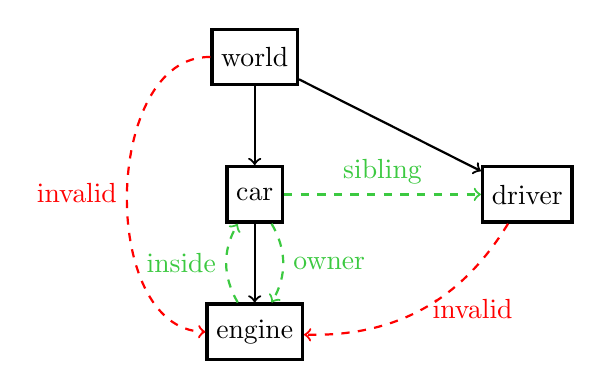
\begin{tikzpicture}[object/.style={rectangle, draw, very thick, minimum size=20}]
    \node[object] (World) {world};
    \node[object] (Car) [below=of World] {car};
    \node[object] (Driver) [right=of Car,xshift=1.5cm] {driver};
    \node[object] (Engine) [below=of Car] {engine};

    \draw[->,thick] (World) to (Car);
    \draw[->,thick] (World) to (Driver);
    \draw[->,thick] (Car) to (Engine);

    \draw[->,thick,dashed,cgreen] (Car) edge[bend left] node[right] {owner} (Engine);
    \draw[->,thick,dashed,cgreen] (Engine) edge[bend left] node[left] {inside} (Car);
    \draw[->,thick,dashed,cgreen] (Car) edge node[above] {sibling} (Driver);
    \draw[->,thick,dashed,red] (World) edge[bend right=90] node[left] {invalid} (Engine);
    \draw[->,thick,dashed,red] (Driver) edge[bend left] node[right] {invalid} (Engine);
  \end{tikzpicture}

  \caption{Owners-as-dominators \cite{flexible-alias-protection}: Solid lines indicate "owns" and dotted lines indicate "references".}
  \label{fig:owners-as-dominators}
\end{figure}

Figure \ref{fig:owners-as-dominators} was adapted from an example by Clarke et al. \cite{flexible-alias-protection} and demonstrates valid (green) and an invalid (red) references in an ownership hierarchy.
Each of the three reference validity rules that were defined previously will be illustrated using this example figure.

\paragraph{Owner}

The object \emph{car} owns the object \emph{engine}, meaning that \emph{car} can validly reference \emph{engine} according to the first rule.

An owner being able to access its owned objects is the most trivial and intuitive rule.

\paragraph{Sibling}

The objects \emph{car} and \emph{driver} are siblings, meaning that they can validly reference each other according to the second rule.

The lack of further rules implies that siblings are the only objects that an object can validly reference besides the objects it owns and the objects it is inside of.
The sibling relationship would, therefore, be used for objects that exist independently but can still interact with each other.

\paragraph{Outside/inside}

The object \emph{engine} is inside the object \emph{car} because \emph{engine} is owned by \emph{car}.
Conversely, \emph{car} is outside \emph{engine}.
Therefore, \emph{engine} can validly reference \emph{car} according to the third rule.

The original Flexible Alias Protection model, which these ownership types are based on, also imposed the restriction "that the only objects that can access [an object] are the object that owns it and other objects inside that [object]" \cite{flexible-alias-protection}.
The implication is that this model only protects objects from external access.
Internally, an object can still access its owner (and its owner's owner etc.).

% TODO: why iterators can be implemented because of 3. outside rule
Dietl and Müller \cite{lightweight-ownership} point out that there exist several slightly different specifications of the owners-as-dominators model.
They claim that Clarke's owners-as-dominators property \cite{ownership-types-survey} is weaker than others "by allowing instances of inner classes to access the representation of the instance of the outer class they are associated with" \cite{lightweight-ownership}, which we have already identified in the third rule.
They state that, thereby, this owners-as-dominators model can handle iterators, but not more general forms of sharing \cite{lightweight-ownership}.

\paragraph{Further implications}

Primarily, these three rules imply that any external reference to an object is only possible through its owner.
This is examplified in Figure \ref{fig:owners-as-dominators} where the object \emph{world} is trying to access the object \emph{engine}, which is not allowed because \emph{world} is neither a direct owner of, a sibling of or inside of \emph{engine}.
Instead, \emph{world} could only reference \emph{engine} through the \emph{engine}'s owner \emph{car}.

According to Dietl and Müller \cite{lightweight-ownership}, the owners-as-dominators model restricts \emph{where} references are allowed to point to.
% TODO: find reference/quote
% Any object that can be validly referenced may be mutated through that reference.

Its strictness can be seen as both an advantage and a disadvantage of the owners-as-dominators model.
The advantage is that the model provides a simple, clear and strong guarantee that allows for reasoning about various properties of the code.
However, it also makes programming more difficult by not allowing common idioms that involve aliasing. \cite{ownership-types-survey}


\subsection{Owners-as-modifiers}
\label{sec:owners-as-modifiers}

Another kind is the \emph{owners-as-modifiers} model \cite{ownership-types-survey}, which is a weaker form of owners-as-dominators that additionally allows read-only references.
A read-only reference can only be used to read files and call \emph{pure methods}.
Pure methods are defined as methods that do not modify the fields of any existing objects. \cite{ownership-types-survey}

For \emph{a} to validly reference \emph{b} through reference \emph{r}, at least one of the following rules \cite{ownership-types-survey} must apply.
\begin{enumerate}
  \item \emph{a} is the owner of \emph{b},
  \item \emph{a} and \emph{b} are siblings, or
  \item \emph{b} is outside of \emph{a}, or
  \item \emph{r} is a read-only reference and only pure methods can be called on it.
\end{enumerate}
We can see that the owners-as-modifiers concept extends the rules specified for owners-as-dominators.
The only additional rule is that a reference can also be valid if it is a read-only reference and only pure methods are being called on it.

\begin{figure}
  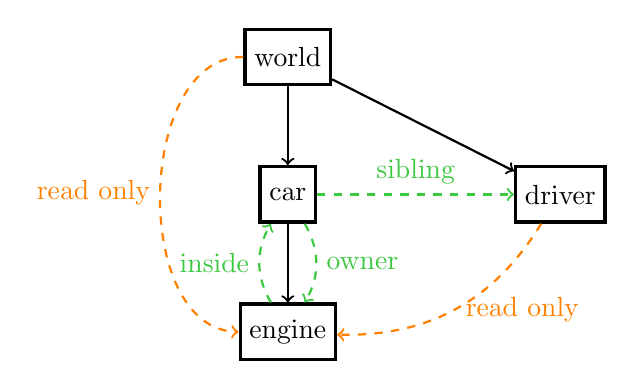
\begin{tikzpicture}[object/.style={rectangle, draw, very thick, minimum size=20}]
    \node[object] (World) {world};
    \node[object] (Car) [below=of World] {car};
    \node[object] (Driver) [right=of Car,xshift=1.5cm] {driver};
    \node[object] (Engine) [below=of Car] {engine};

    \draw[->,thick] (World) to (Car);
    \draw[->,thick] (World) to (Driver);
    \draw[->,thick] (Car) to (Engine);

    \draw[->,thick,dashed,cgreen] (Car) edge[bend left] node[right] {owner} (Engine);
    \draw[->,thick,dashed,cgreen] (Engine) edge[bend left] node[left] {inside} (Car);
    \draw[->,thick,dashed,cgreen] (Car) edge node[above] {sibling} (Driver);
    \draw[->,thick,dashed,orange] (World) edge[bend right=90] node[left] {read only} (Engine);
    \draw[->,thick,dashed,orange] (Driver) edge[bend left] node[right] {read only} (Engine);
  \end{tikzpicture}

  \caption{Owners-as-modifiers \cite{ownership-types-survey}: Solid lines indicate "owns" and dotted lines indicate "references".}
  \label{fig:owners-as-modifiers}
\end{figure}

\paragraph{Implications}

Dietl and Müller \cite{lightweight-ownership} suggest that the owners-as-modifiers approach allows references to point to objects in arbitrary contexts, but restricts \emph{how} references can be used.
In particular, any object can be referenced by any given object.
However, only an object that is the owner of, a sibling of or inside of another given object may receive a reference to that object that allows mutating the object.
Figure \ref{fig:owners-as-modifiers} demonstrates that all other objects, such as \emph{world} or \emph{driver}, which may not be allowed to obtain a mutable reference to an object for the reasons above, can still receive read access to said object.

% TODO: find better disadvantage
A disadvantage of the model may be the added complexity of read-only references.
However, its advantage is that it expands the programming possibilities of the owners-as-dominators principle and fulfills the requirements needed for the verification of the functional correctness of object-oriented programs.


% \subsection{Limitations}
% \subsection{From theory to Rust}

% These early ownership type models carry some flaws with them.
% For example, in a system using the owners-as-dominators approach, one cannot programmatically create iterators.

% TODO: chapter 6 of ownership-types-survey


\section{Implementation in Rust}
\label{sec:implementation-in-rust}

Rust's notion of ownership is the culmination of a long line of work.
Wadler [1991] and Baker [1992] originally aimed to develop systems for functional programming without garbage collection.
% TODO: pervasive synonym
However, as noted by Wakeling and Runciman [1991], Wadler's effort relied greatly on pervasive copying.
The associated performance overhead of a reliance on copying was too large for use in real-world systems programming efforts.
Thus, it is best understood that Rust's ownership model is based off of Baker's work on Linear Lisp where linearity enabled efficient reuse of objects in memory [Baker 1992, 1994a,b,1995].
The resemblance is especially strong between Rust \emph{without} borrowing and Baker's 'use-once' variables [Baker 1995].
\cite{oxide}
% TODO: explain use-once concept in more detail with reference to Baker's paper

However, techniques like the 'use-once' variables [Baker 1995] differentiate themselves from Rust by requiring that all objects must be managed uniquely.
Instead, Rust allows the programmer to use unique references [Minsky 1996] with unguarded mutation or to use shared references without mutation.
This flexibility in choosing arises at the point where the programmer creates a new reference, and draws inspiration from work on ownership types and flexible alias protection [Clarke et al. 1998; Noble et al. 1998].

One can argue that Rust's ownership system is an extended version of the ownership model \emph{owners-as-modifiers}.
% In Rust, like in owners-as-modifiers, an object can reference any other given object with read access.
The Rust and owners-as-modifiers approaches differentiate themselves from the owners-as-dominators model, since they both allow read-only references to any object.
However, as will be discussed further in \ref{sec:rust-references}, Rust allows both read-only and mutable references in a controlled manner.
This allows for expressing many more programming idioms.

Furthermore, we can link certain owners-as-modifiers concepts to concepts from Rust.
Firstly, siblings...


% TODO: question: can an object access owned children transitively? How is it in Rust (if someone asks me this question)?

Most of the Rust-related information gathered in this chapter is derived from the "Understanding Ownership" section from the Rust Book \cite{rust-book}.
If anything was retrieved from other sources, it would be cited as such.


% \subsection{From theory to Rust}
% \label{sec:use-once-variables}

% TODO: fix this section by reformatting the copied text and adding quotes from the references

% Rust's notion of ownership rests atop a long lineage of work, harkening back to the early days of linear logic [Girard 1987], and especially efforts by Wadler [1991] and Baker [1992] to develop systems for functional programming without garbage collection.
% However, as noted by Wakeling and Runciman [1991], Wadler’s effort relied greatly on pervasive copying.
% This reliance on copying and the associated performance penalty would not suffice for real world systems programming efforts, and thus, Rust’s ownership model is best understood as instead building off of Baker’s work on Linear Lisp where linearity enabled efficient reuse of objects in memory [Baker 1992, 1994a,b,1995].
% The resemblance is especially strong between Rust without borrowing and Baker’s ’use-once’ variables [Baker 1995].

% Rust’s main departure from techniques like ’use-once’ variables [Baker 1995] is a softening of a rather stringent requirement: namely, that everything must be managed uniquely.
% Instead, Rust allows the programmer to locally make a decision to use unique references [Minsky 1996] with unguarded mutation or to use shared references without such mutation.
% This flexibility in choosing arises at the point where the programmer creates a new reference, and draws inspiration fromwork on ownership types and flexible alias protection [Clarke et al. 1998; Noble et al. 1998].



% \subsection{How Rust implements ownership types}
% \label{sec:rust-ownership-types}

% The modern programming language Rust uses an extended version of the ownership type model \emph{owners-as-modifiers}.
% In addition to read-only references, which are allowed in owners-as-modifiers, Rust also supports mutable references in a controlled manner.


\subsection{Memory allocation system}
\label{sec:memory-allocation}

There are two major requirements that a memory allocation system must fulfill:
At runtime, memory can be requested from the memory allocator, and there exists a mechanism for memory to be freed by the memory allocator.

The first requirement is trivial.

% TODO: find source for both garbage collection and manual freeing
One possible implementation of the second requirement is using a garbage collector, which keeps track of and cleans up memory that is no longer used.
% TODO: find source for GC disadvantages
This, however, has a runtime performance overhead and can lead to a non-deterministic cleanup of resources.

% TODO: find source for manual free disadvantages
Another more traditional solution is requiring memory to be freed explicitly.
This is a notorious source of bugs.
If memory is never freed because it was forgotten, memory is wasted.
If it is freed multiple times or accessed again after having been freed, it will result in undefined behavior.

The ideal solution pairs one \emph{allocate} with exactly one \emph{free}.
Rust uses neither a garbage collector nor requires memory to be freed manually.
Instead, the concept of ownership is leveraged to determine when to free memory.

The Rust Book \cite{rust-book} defines ownership as a set of rules that govern how it manages memory.
The compiler checks whether these rules are adhered to and does not compile the program if they are violated.
The ownership rules in Rust are as follows:
\begin{enumerate}
  \item Each value in Rust has an owner.
  \item There can only be one owner at a time.
  \item When the owner goes out of scope, the value will be \emph{dropped}.
\end{enumerate}
The scope of a value is the range within a program in which it is valid.
Rust automatically calls the function \emph{drop} when a value goes out of scope, which frees the associated memory.

The following describes how the concept of ownership is implemented in Rust.


% TODO: wording of value and types used interchangedly here, maybe incorrect
\subsection{Transferring ownership}
\label{sec:rust-transferring-ownership}

One common restriction to the early ownership systems is that the owner of an object must be set upon creation and then fixed for the lifetime of the object \cite{ownership-types-survey}.
Rust extends the original ownership concepts by allowing the ownership of an object to be transferred.

First, one must differentiate between values that are stored on the stack and those stored on the heap.
In Rust, primitive data types (e.g. signed 32-bit integers \emph{i32}) are stored on the stack since their sizes are small and known at compile time.
In contrast, values are stored on the heap if their size is dynamic and, therefore, unknown at compile time.
The ownership concepts in Rust mainly apply to values stored on the heap.

\paragraph{Heap-based variables}

In addition to the memory safety that ownership types provide, ownership transfers can also reduce redundant copy operations.
Since heap-based values could be arbitrarily large at runtime, copying the whole value instead of transferring ownership could be very inefficient.
There are several different scenarios in which ownership is transferred.

In the simplest scenario, ownership is transferred from the variable \emph{a} to the variable \emph{b} when \emph{b} is assigned to \emph{a}.
\footnote{In some code snippets, the main function is omitted for the sake of simplicity}

\begin{lstlisting}
let a = HeapBasedType::default();
let b = a;
\end{lstlisting}
In Rust terminology, \emph{a} is \emph{moved} into \emph{b}.
After the move, \emph{a} is no longer valid, and \emph{b} is the new owner of the value.

Heap-based values will always be generated by a function at runtime.
In the above example, the return value of the function \verb|HeapBasedType::default()| is moved into \emph{a}.
Furthermore, one can generalize the above scenario to ownership being transferred from the variable \emph{a} to the variable \emph{b} when \emph{b} is assigned to the return value \emph{a} of \emph{foo}.
\begin{lstlisting}
fn main() {
  let b = foo();
}
fn foo() {
  let a = HeapBasedType::default();
  a
}
\end{lstlisting}

Lastly, ownership is transferred from the variable \emph{a} to the variable \emph{b} when \emph{a} is passed to function \emph{foo}, which takes a parameter \emph{b}.
\begin{lstlisting}
fn main() {
  let a = HeapBasedType::default();
  foo(a);
}
fn foo(b: HeapBasedType) {
  // do something with b
}
\end{lstlisting}
In \emph{foo}, \emph{b} is the owner of the value until it is \emph{dropped} at the end of the function.
Accessing the previous owner of a value after the ownership of that value has been transferred elsewhere will lead to a compile-time error.
In this case, trying to access \emph{a} after line 3 would not compile, as \emph{a} is no longer the owner of the value.

The heap-allocated \emph{String} type in Rust provides a good example demonstrating ownership transfer of heap-based values.
\begin{lstlisting}
let x: String = String::from("hello world");
let y: String = x;
println!("x: {}, y: {}", x, y);
\end{lstlisting}
After \emph{x} is moved into \emph{y} in line 2, \emph{x} is no longer valid.
Therefore, Rust prevents you from accessing the invalid \emph{x} in the third line, and the program will not compile.


\paragraph{Stack-based values}

In contrast to heap-based values, the size of stack-based values is known at compile time and is usually small.
Therefore, stack-based values in Rust are \emph{copied} instead of \emph{moved}.
% TODO: explain copy trait
Internally, this works because primitive types are annotated with the \emph{Copy} trait.

Besides the heap-allocated \emph{String} type, Rust also supports string literals \emph{\&str}, which are stored on the stack.

The following piece of code \cite{rust-book}, which is similar to the code from above but replaces the \emph{String} type with string literals, demonstrates how stack-based string literals are \emph{copied} instead of \emph{moved} into other variables in Rust.
\begin{lstlisting}
let x: &str = "hello world";
let y: &str = x;
println!("x: {}, y: {}", x, y);
\end{lstlisting}
The value of \emph{x} is copied into \emph{y}, after which both variables are still valid.
Therefore, the program compiles and "x: hello world, y: hello world" is printed to stdout.


\paragraph{Moving fields out of structs}

In their work on the owners-as-modifiers property, Clarke et al. \cite{ownership-types-survey} emphasize that rather than simply protecting the fields of an object from external access, ownership types also protect the objects stored in the fields, thereby enabling an object to claim (exclusive) ownership of and access to other objects.
This notion has been implemented in the Rust ownership system as well.
The following example illustrates how not only whole objects, but also fields (called \emph{structs} in Rust terminology), can be moved into other objects.

\begin{lstlisting}
struct Car {
  engine: Engine,
}
fn main() {
  let car = Car::default();
  let moved_engine = car.engine; // valid
  car.drive() // error: use of partially moved value: 'car'
}
\end{lstlisting}

% TODO


\subsection{The Clone trait}
\label{sec:rust-clone-trait}

By default and by design, Rust will never automatically create deep copies of data stored on the heap.
To do so, one must explicitly call the \emph{clone} method on an object.

The following adjustment to the code snippet from above creates a deep copy of \emph{x} and compiles successfully.
\begin{lstlisting}
let x: String = String::from("hello world");
let y: String = x.clone();
println!("x: {}, y: {}", x, y);
\end{lstlisting}


\subsection{Immutability}
\label{sec:rust-immutability}

By default, all values and references in Rust are immutable.
An object is defined as immutable if its state cannot be modified after its creation.
In Rust, mutable values and references must be explicitly created using the \emph{mut} keyword.

For example, a string literal can be appended to a mutable String.
\begin{lstlisting}
let mut s = String::from("hello");
s.push_str("hello");
\end{lstlisting}


\subsection{References and borrowing}
\label{sec:rust-references}

Object aliasing has already been defined as the concept of accessing the same memory through different symbolic names.
Specifically, the \emph{owners-as-modifiers} approach relies on implementing the aliasing concept.
Therefore, any programming language based on this form of ownership type must provide a way of achieving this behavior.
One way to implement this behavior is by allowing the use of \emph{pointers}, which are commonly used in low-level programming languages.
However, even though they exist, "working with raw pointers in Rust is uncommon [and] typically limited to a few patterns" \cite{rust-pointer-documentation}.
% Instead, Rust primarily uses \emph{references} as the preferred way of implementing aliasing.
Instead, Rust uses \emph{references} as the preferred way of implementing aliasing.

In Rust, a \emph{reference} is an address that points to a value that is owned by another variable.
Unlike traditional \emph{pointers}, a reference is guaranteed by the compiler to point to a valid value.
In Rust terminology, creating a reference is called \emph{borrowing}.
A reference does not own the value it points to.
Therefore, only the reference itself, not the value that the reference has borrowed, is dropped at the end of the reference's scope.
Borrowing is useful for performing an operation on a value without taking ownership of it.

Rust supports creating both immutable and mutable references.
The scope of a reference starts where it is introduced and extends until the last time it is used.

\paragraph{Immutable references}

Immutable references can be seen as read-only references and are acquired using the \emph{\&} operator.
The value that immutable references refer to may not be modified.
Otherwise the program will not compile.

\begin{lstlisting}
fn main() {
  let s = String::from("hello");
  let r1 = &s;
  let r2 = &s;
  print_str(r1);
  print_str(r2);
}
fn print_str(s: &String) {
  println!("printed from a reference: {}", s);
}
\end{lstlisting}

The program will compile as long as the value \emph{s} is not modified in the \emph{print\_str} function.
Furthermore, an unlimited amount of immutable references to the same value may exist at any time.
The scopes of each of these immutable references may overlap.
However, mutable references provide an exception to this rule, which is explained in the next section.

Multiple immutable references are allowed because none of the references can modify the value.
Thereby, no immutable reference can affect another reference's reading of the value.


\paragraph{Mutable references}

Rust also supports mutable references, which are created with the \emph{\&mut} keyword and allow the borrowed value to be modified.
For obvious reasons, creating a mutable reference is only possible if the borrowed value is also mutable.

\begin{lstlisting}
fn main() {
  let mut s = String::from("hello");
  modify_str(&mut s);
}
fn modify_str(s: &mut String) {
  s.push_str(" world");
}
\end{lstlisting}

The scope of a mutable reference to a value may not overlap with the scope of any other immutable or mutable reference to that same value.
This implies that there may only exist one mutable reference to a value at any given time.
During this time, no further immutable or mutable references are allowed.

This restriction exists to identify and prevent \emph{data races}, which can cause undefined behavior at compile time.
A data race occurs when two or more pointers access the same data simultaneously, at least one of the points is being used to write the data, and there exists no mechanism to synchronize access to the data \cite{rust-book}.

However, the following code example \cite{rust-book} shows that it is important to note that the creation of multiple mutable and immutable references with scopes that do not overlap is allowed.

\begin{lstlisting}
let mut s = String::from("hello");

let r1 = &s; // allowed
let r2 = &s; // allowed
println!("{} and {}", r1, r2);

let r3 = &mut s; // allowed
r3.push_str(" world");
println!("{}", r3);
\end{lstlisting}

Since \emph{r1} and \emph{r2} are not used after line 5, that is where their scopes end.
The scope of the mutable reference \emph{r3} only starts in line 7.
Therefore, the scopes of the mutable reference and the two immutable references do not overlap, and the program compiles.

% \paragraph{Lifetimes}

% TODO: explain how dangling references are prevented



% \paragraph{Limits of the ownership approach}

% TODO: explain how rust uses unsafe code to implement std library
% discuss limitations of ownership types: any structures that need raw pointers? how can one deal with them?

% Rust's std lib is largely implemented using unsafe code (that doesn't strictly follow the ownership rules) for performance reasons (I think, maybe there are also other reasons).
% If the ownership semantics are no longer used to prove the correctness of a program, how is the safety of the std lib guaranteed?
% Is it guaranteed at all?
% If not, a compelling argument for ownership types with an unsafe implementation is still, that the programmers rarely/never have to use the unsafe code, and will make less mistakes.
% The API of the stdlib is safe, the implementation isn't.



% \section{Other ownership implementations}

% TODO: compare implementation of ownership types to other languages
% It is not trivial to compare the implementation of the ownership concept of Rust with that of another programming language because Rust is kind of the only one doing so.
% CPP is a good candidate

% - comparison to alternative type systems without ownership (C/C++: none at all, Java: garbage collection)
% - choose non-ownership programming language e.g. C++20
% - compare code examples
% - compile time differences between Rust and non-ownership lang
% - runtime differences between Rust and non-ownership lang


\section{Summary \& Outlook}
\label{sec:summary}

In summary, programming languages based on ownership types can eliminate many aliasing-related issues by enforcing strict rules on the existence and behavior of references to values.
The owners-as-dominators and owners-as-modifiers models enforce different levels of strictness on both where and how references may be used.
Furthermore, an enhanced version of the ownership concept is integral to the Rust programming language.
Compared to more commonly used low-level programming languages like C, Rust introduces many memory-related rules that are strictly enforced by the compiler at compile time, allowing for safe runtime performance and omitting the need for many manual, rigorous and error-prone memory reference checks that programmers used to have to perform.
Even though the Rust compiler forces developers to think more intentionally about how they deal with memory through ownership, they will receive helpful compile-time error messages instead of crashes or undefined behavior at runtime if they do something wrong.

It will be interesting to see how Rust's development will continue in the future.
Given its rise in popularity as a safe and performant programming language using strict ownership types, the question arises of whether ownership types might also be incorporated into more new or existing programming languages in the future.


\bibliographystyle{ACM-Reference-Format}
\bibliography{paper} % read paper.bib file

\end{document}
